\documentclass{ltjsarticle}
\usepackage{luatexja-otf}
\usepackage[]{luatexja,luatexja-fontspec}\usepackage{booktabs}
\usepackage{array}
\usepackage{graphicx}
\usepackage{mathpazo}
\usepackage{amsmath}
\usepackage{amsthm}
\usepackage{amssymb}
\usepackage{amsfonts}
\usepackage[noheadfoot,top=0mm,bottom=0mm,hmargin=-5mm]{geometry}
\usepackage{tikz}
\usetikzlibrary{matrix}
\usepackage{pgfcore}
\usepackage{color}
\newtheorem{dfn}{Def}
\newtheorem{thm}{Thm}
\newtheorem{cor}{Cor}
\newtheorem{prop}{Prop}
\newtheorem{rk}{remark}
\newtheorem{claim}{claim}
\newtheorem{recall}{recall}
\newtheorem{ques}{Q.}
\date{\today}
\author{俺}
\title{テスト}
\begin{document}\maketitle
\section{test.md}

\section{テスト}

\begin{itemize}
\item
  テスト
\item
  いろは
\item
  にほへと
\item
  画像テスト
\end{itemize}

\begin{center}
  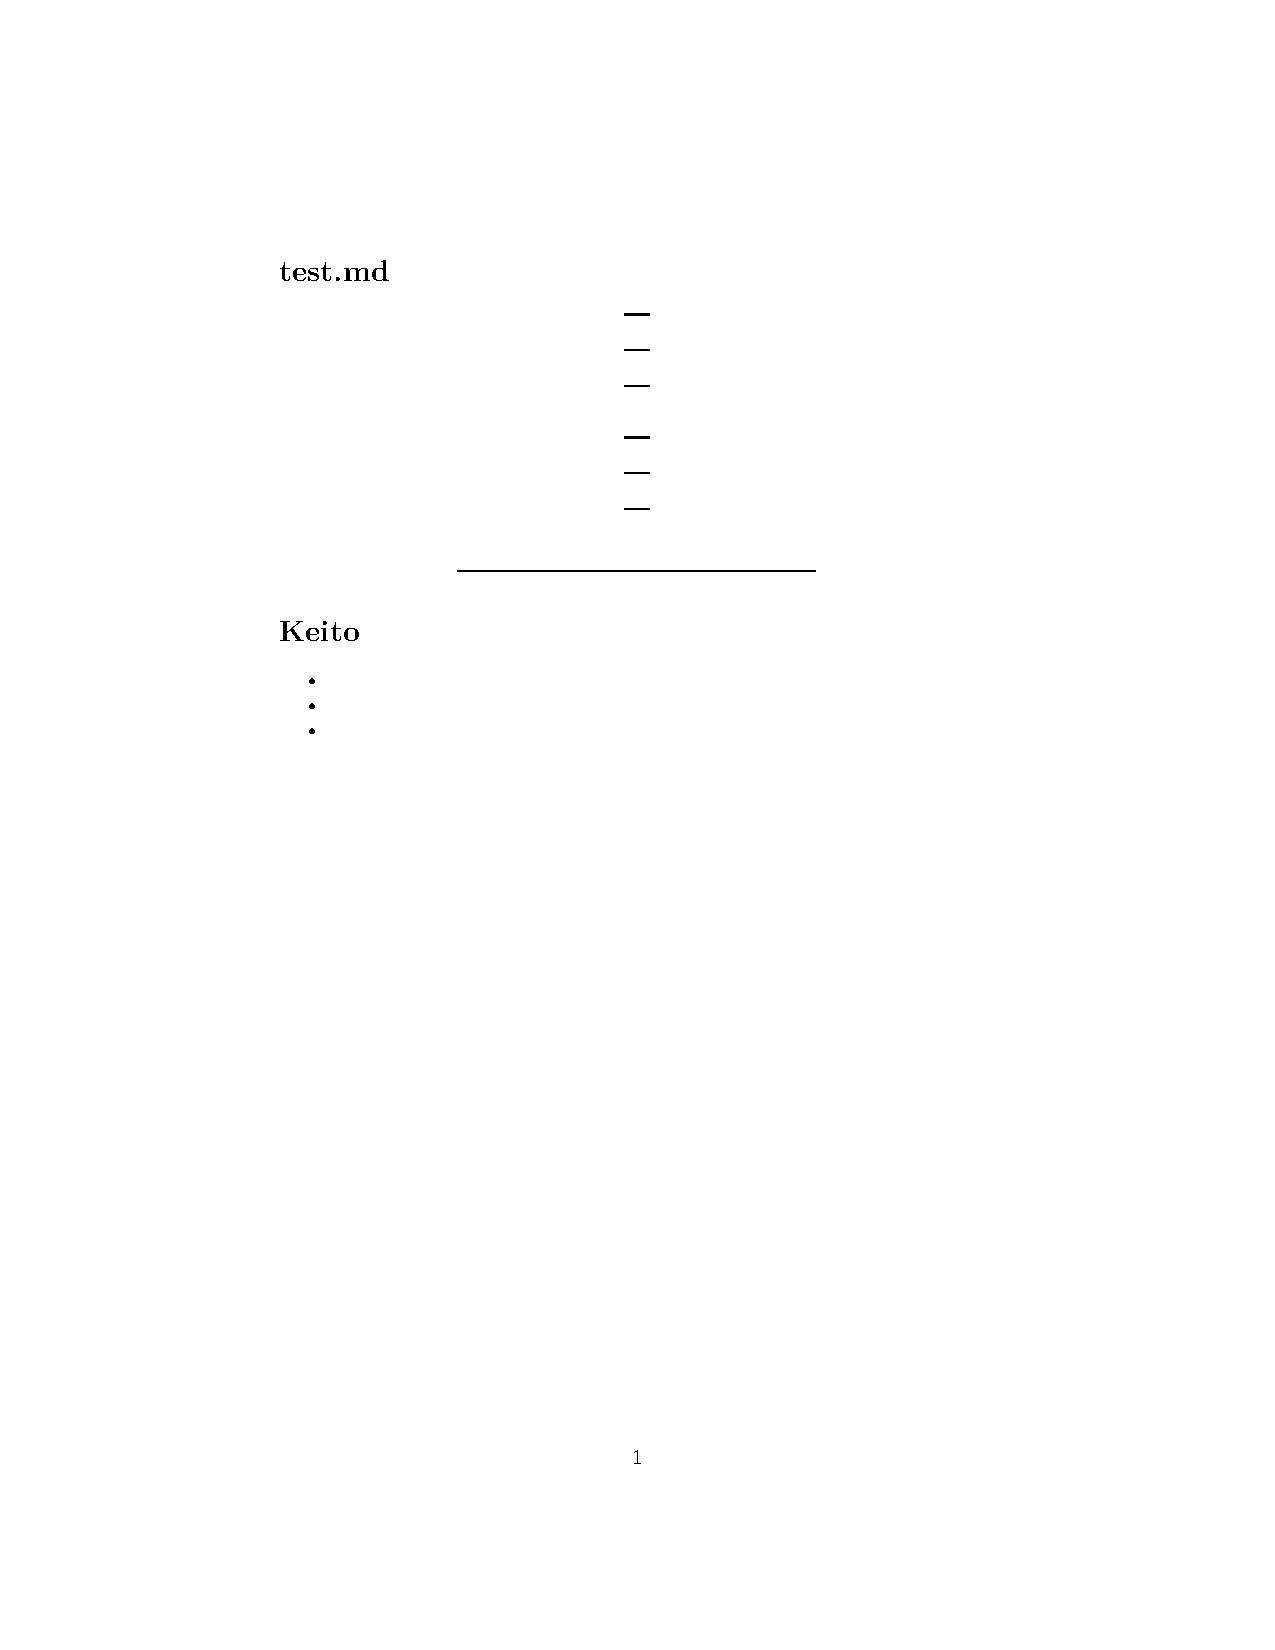
\includegraphics{example.pdf}
\end{center}
\end{document}
